\documentclass[hidelinks,a4paper, 11pt, nofootinbib]{article}
\usepackage[width=15.5cm, left=3cm, top=2.5cm, right=2cm, left=2cm, height= 24.5cm]{geometry}
\usepackage[spanish, es-tabla]{babel} %es-tabla es para que ponga Tabla en vez de Cuadro en el caption
\usepackage[utf8]{inputenc}
\usepackage[T1]{fontenc}
\usepackage{xspace}
\usepackage{xargs}
\usepackage{fancyhdr}
\usepackage{lastpage}
\usepackage{caratula}
\usepackage[bottom]{footmisc}
\usepackage{amsmath}
\usepackage{amssymb}

\usepackage{float}% http://ctan.org/pkg/float

\usepackage{algorithm}
\usepackage[noend]{algpseudocode}
\usepackage{array}
\usepackage{xcolor,colortbl}
\usepackage{amsthm}
\usepackage{listings}

\usepackage{pgf}
\usepackage{tikz}
\usetikzlibrary{arrows,automata}

\usepackage{graphicx}
\usepackage{sidecap}
\usepackage{amsmath}
\usepackage{wrapfig}
\usepackage{caption}

\usepackage{hyperref}
\hypersetup{
  colorlinks   = true, %Colours links instead of ugly boxes
  urlcolor     = blue, %Colour for external hyperlinks
  linkcolor    = blue, %Colour of internal links
  citecolor   = red %Colour of citations
}

\usepackage{comment}

\usepackage[
  backend=bibtex,
  style=alphabetic
]{biblatex}
\addbibresource{bibliografia.bib}


\captionsetup[table]{labelsep=space}


\setlength{\parindent}{1em}
\setlength{\parskip}{0em}

%Defino colores para las tablas
\definecolor{LightCyan}{rgb}{0.77,0.9,0.9}
\definecolor{Gray}{gray}{0.8}
\definecolor{azul}{HTML}{0040C0}
\definecolor{rojo}{HTML}{FD0A10}


%%fancyhdr
\pagestyle{fancy}
\thispagestyle{fancy}
\addtolength{\headheight}{1pt}
\lhead{Algoritmos y Estructuras de Datos 3 - TP1}
\rhead{$1^{er}$ cuatrimestre - 2017}
\cfoot{\thepage\ / \pageref{LastPage}}
\renewcommand{\footrulewidth}{0.4pt}
\renewcommand{\labelitemi}{$\bullet$}

%%caratula
\materia{Algoritmos y Estructuras de Datos III}
\titulo{Trabajo Práctico 1}
%\subtitulo{}
%\grupo{Grupo 12}
\integrante{Seijo, Jonathan Adrián}{592/15}{jon.seijo@gmail.com}

\fecha{Abril 2017}

\usepackage{etoolbox}
\AtBeginEnvironment{tikzpicture}{\shorthandoff{>}\shorthandoff{<}}{}{}

\begin{document}

\maketitle
\tableofcontents

\newpage

\section{Introducción}
Dada una secuencia de números $A$, se quiere pintar algunos de sus números de color rojo o azul. Dicho de otro modo, cada número de la secuencia puede ser pintado de color rojo, azul o de ningun color. \\

La secuencia $A$ puede ser pintada de muchas formas diferentes, pero no todas son válidas. \\ 
% Más formalmente, 
% $(\forall e \in A), $ color($e$) $\in$ $\{$Rojo, Azul, Ninguno$\}$ 
Decimos que una secuencia es valida si se cumple las siguientes condiciones:
\begin{enumerate}
\item Todos los elementos de color \textcolor{red}{rojo} estan ordenados de forma estrictamente creciente 
\item Todos los elementos de color \textcolor{blue}{azul} estan ordenados de forma estrictamente decreciente 
\end{enumerate}



\newpage
\section{Backtracking}
\subsection{Solución naive}

Llamo $A$ a la secuencia de números que quiero pintar, y $n$ a la cantidad de elementos en $A$. De todas las secuencias válidas de colores que puedo formar quiero saber cual es la mínima cantidad de elementos que puedo dejar sin pintar. \\

Una forma natural de pensar la solución es la siguiente: genero todas las formas de pintar posibles, y veo cual es el mínimo sin pintar que puede usarse para las secuencias que son válidas. Esa es la idea central detrás de ambos algoritmos de backtracking. Veamos entonces una posible implementación, la forma \textit{naive}. \\

El primer elemento puede ser Rojo, Azul o Ninguno. Dado el color del primero, el segundo elemento puede también ser Rojo, Azul o Ninguno. Fijados el primero y el segundo, el tercero puede ser tomar cualquiera de las tres posibilidades, y así siguiendo. \\

Una vez fijos los colores de los $n$ elementos, reviso si la secuencia de colores que se formó es válida. (Esto es, que los elementos rojos estén ordenados crecientemente y los azules decrecientemente, ambos de forma estricta). \\

Si la secuencia formada era válida, entonces cuento la cantidad de elementos sin pintar, y devuelvo ese número. La respuesta final es se consigue tomando el mínimo de todos los mínimos. \\

Como detalle de implementación, en caso de que la secuencia formada no sea válida, devuelvo un valor infinito para que no afecte al valor mínimo solución. Esta solución existe porque no pintar ningún elemento de ningún color es siempre una solucion válida \textbf{finita}


\subsection{Pseudocódigo}

\begin{algorithm}[H]
\begin{algorithmic}
\Procedure{backtrack}{secuencia(Colores) $colores$, int $actual$}

\If {$actual = n$}

  \If {EsValido($colores$)}
    \State return CantSinPintar($colores$)
  \Else
    \State return $\infty$
  \EndIf

\Else

  \State colores[$actual$] $\gets$ Rojo
  \State $minimoConRojo$ $\gets$ backtrack($colores$, $actual + 1$) \\

  \State colores[$actual$] $\gets$ Azul
  \State $minimoConAzul$ $\gets$ backtrack($colores$, $actual + 1$) \\

  \State colores[$actual$] $\gets$ Ninguno
  \State $minimoSinPintar$ $\gets$ backtrack($colores$, $actual + 1$) \\

  \State return Min($minimoConRojo$, $minimoConAzul$, $minimoSinPintar$)

\EndIf
\EndProcedure
\end{algorithmic}
\end{algorithm}


Auxiliares:

\begin{algorithm}[H]
\begin{algorithmic}
\Procedure{EsValida}{secuencia(Colores) $colores$}

    \State bool $rojoValido$ $\gets$ EsCreciente(DameRojos($colores$))  \Comment $O(n)$
    \State bool $azulValido$ $\gets$ EsDecreciente(DameAzules($colores$)) \Comment $O(n)$
    \State return ($rojoValido \land azulValido$)

\EndProcedure
\end{algorithmic}
\end{algorithm}


\begin{algorithm}[H]
\begin{algorithmic}
\Procedure{CantSinPintar}{secuencia(Colores) $colores$}
    \State return Tamaño(DameSinPintar($colores$))  \Comment $O(n)$
\EndProcedure
\end{algorithmic}
\end{algorithm}


Para resolver el problema original, llamo a la función con los siguientes parámetros:

\begin{algorithm}[H]
\begin{algorithmic}
\Procedure{Resolver naive}{secuencia(int) $A$}
  \State backtrack($secuenciaColoresVacia(n)$, $0$)
\EndProcedure
\end{algorithmic}
\end{algorithm}


\subsection{Complejidad}

El algoritmo presentado visita todas las posibles combinaciones de colores. Cada uno de los elementos tiene tres posibilidades, y como hay $n$ elementos, la cantidad de combinaciones posibles es $3^{n}$. Por lo tanto, visitar todas las posibilidades es $O(3^{n})$.

Además, para cada combinación, se revisa en $O(n)$ si es una secuencia valida o no. Por lo tanto, la complejidad total del algoritmo es $O(n * 3^{n})$ \\

Otra forma de verlo es pensando en el arbol de recursión que se va formando al llamar a la función. Cada nivel representa al elemento iésimo de $A$, y cada nodo representa el color del elemento. De todo nodo se desprenden tres posibilidades hasta llegar al nivel $n$. Al llegar a una hoja, se decide si la secuencia \textit{hasta esa hoja} es válida, en tiempo lineal. \\

Sabiendo que en un árbol ternario el nivel \textbf{i} tiene $3^{i}$ nodos, y sabiendo que el arbol tiene $n$ niveles, la cantidad de nodos que se visitan es: \\

$$\sum_{i = 0}^{n} 3^{i} = \frac{3^{n+1}}{2} = O(3^n)$$

El costo de las visitas de nodos no es el total, pues para cada una de las hojas se verifica si la secuencia obtenida es válida o no. Las hojas se encuentran en el útimo nivel $n$, entonces el árbol de recursión tiene $3^n$ hojas, donde cada hoja tiene costo $O(n)$. El costo de operar en las hojas entonces es $3^n * O(n) = O(n * 3^n)$ \\

El costo \textbf{total} es la suma entre visitar todos los nodos y operar en las hojas, es decir:

$$O(3^n) + O(n * 3^n) = O(n * 3^n) $$


\subsection{Solución con poda}

El algoritmo anterior funciona, pero puede mejorarse si tenemos en cuenta algunas observaciones:

\begin{enumerate}
\item Pueden filtrarse las secuencias válidas a medida que vamos construyendo la secuencia de colores.
\item Recorriendo de izquierda a derecha, lo único que se necesita para saber si es válido pintar cierto elemento de algun color, es ver el valor del último elemento antes del actual que fue pintado de ese mismo color.
\item Puede conocerse la cantidad de elementos sin pintar a medida que se va pintando la secuencia.
\item La cantidad de elementos sin pintar \textbf{no} aumenta si se pinta rojo o azul.
\item Si la cantidad de elementos sin pintar es mayor al mínimo entontrado, entonces no vale la pena seguir explorando esa secuencia, pues la cantidad de elementos sin pintar no puede disminuir.
\end{enumerate}

\subsection{Pseudocódigo}

Siguiendo la idea principal del algoritmo anterior, pero teniendo en cuenta las nuevas ideas, podemos mejorar nuestro algoritmo:

\begin{algorithm}[H]
\begin{algorithmic}
\Procedure{backtrack}{int $actual$, int $ultRojo$, int $ultAzul$, int $cantSinPintar$}

\If {$actual = n$}
    \State $minimoTotal \gets cantSinPintar$
    \State return $minimoTotal$
\Else

  \If {($ultRojo = n) \lor (A[actual] > A[ultRojo])$}
    \State $minRojo \gets$ backtrack($actual + 1$, $actual$, $ultAzul$, $cantSinPintar$)
  \EndIf \\

  \If {($ultAzul = n) \lor (A[actual] < A[ultAzul])$}
    \State $minAzul \gets$ backtrack($actual + 1$, $ultRojo$, $actual$, $cantSinPintar$)
  \EndIf \\

  \If{$cantSinPintar + 1 < minimoTotal$}
    \State $minSinPintar \gets$ backtrack($actual + 1$, $ultRojo$, $ultAzul$, $cantSinPintar + 1$)
  \EndIf \\

  \State return Min($minimoConRojo$, $minimoConAzul$, $minimoSinPintar$)

\EndIf
\EndProcedure
\end{algorithmic}
\end{algorithm}



Para resolver el problema original, llamo a la funcion con los siguientes parámetros:

\begin{algorithm}[H]
\begin{algorithmic}
\Procedure{Resolver poda}{secuencia(int) $A$}
  \State backtrack($0$, $n$, $n$, $0$)
\EndProcedure
\end{algorithmic}
\end{algorithm}

Como detalle de implementación, cuando el último rojo (o azul) es $n$, significa que no hay ningún rojo (o azul) aún, porque los índices del arreglo comienzan en cero.

\subsection{Complejidad con poda}

Haciendo un análisis similar al del algoritmo naive, pensando en el arbol de recursión, tenemos que como cota superior se visitan todos los nodos del árbol. La validez de la secuencia se comprueba a medida que se desciende en la recursión, pues no se entra al siguiente paso si la propiedad de los colores no se cumple. Además, se va contando la cantidad de elementos sin pintar a medida que se eligen colores, por lo que tampoco se usa tiempo en eso. \\

Como todo el costo se encuentra en la cantidad de nodos que se visita, y como la cantidad máxima de nodos es $O(3^{n})$, el costo de obtener la respuesta usando este algoritmo con poda en peor caso es $O(3^n)$, mejorando la complejidad del anterior.


\newpage
\section{Programación Dinámica}
\subsection{Solución bottomup}

Generar todas las combinaciones es muy caro computacionalmente. Se puede conseguir algo mejor si pensamos el problema desde otro ángulo. \\

Supongamos que para todo ($i$, $j$) ya tenemos el valor mínimo de elementos sin pintar dado que el $i$-ésimo es el último rojo y el $j$-ésimo es el último azul. De este modo, lo único que tendríamos que hacer es tomar el mínimo de todas las combinaciones de los últimos rojos y azules. Esto es así porque de todas las posibles soluciones para un último rojo y último azul fijos, hay una combinación que es óptima, y es ésta la que nos interesa obtener. \\

Entonces nuestro problema se reduce a: suponiedo que la secuencia tiene el último rojo y el último azul en posiciones fijas, ¿cuál es la mínima cantidad de elementos sin pintar que podemos obtener? \\

Llamo DP[$i$][$ur$][$ua$] a la mínima cantidad sin pintar hasta $A$[$i$] siendo que el elemento en $ur$ es el último rojo y el elemento en $ua$ es el último azul. (Si $ur$ o $ua$ es $n$, represento que no hay rojo o azul) \\

La idea es ir llenando la matriz DP en orden, para encontrar los valores minimos hasta llegar a $i = n$. \\

En los casos base donde $i$ es 0, lleno la matriz con ceros. \\

Veamos ahora DP[$i$][$ur$][$ua$] para el elemento en la posición $i$ (dados un $ur$ y un $ua$) existen 3 casos \\

- \textbf{No lo pinto}: En este caso, la cantidad de elementos sin pintar \textbf{aumenta en uno} con respecto al mínimo hasta $i-1$. Es decir, la solución es igual a $1 + $DP[$i-1$][$ur$][$ua$] \\

- \textbf{Pinto $i$ de rojo}: 
\begin{enumerate}
\item Si $i$ es el último rojo, o si es posible que $i$ sea color rojo (pues no rompe la propiedad) entonces la solución es la misma que la solución hasta $i-1$ siendo que $i$ es el último rojo. Es decir, es igual a DP[$i-1$][$i$][$ua$]
\item Si estoy en la rama donde no hay rojo ($ultRojo = n$), o si estoy en la rama donde el último azul era $i$, entonces no puede ser que $i$ sea rojo, por lo que no hay solución. (Devuelvo $\infty$)
\item Si no era posible que $i$ sea rojo, entonces no hay solucion para este caso. (Devuelvo $\infty$)
\end{enumerate} 

- \textbf{Pinto $i$ de azul}:  Análogo al caso de pintar con rojo  \\

Cuando termina la iteración, DP[$i$][$ur$][$ua$] contiene el mínimo de los tres casos. En todos los casos, sé que el óptimo anterior que utilizo para calcular la solución actual ya está calculado porque los voy calculando en orden. \\

La solución total del problema, es el mínimo valor hasta $i = n$ considerando todas las combinaciones de $ur$ y $ua$.

\subsection{Pseudocódigo bottomup}

\begin{algorithm}[H]
\begin{algorithmic}
\Procedure{Resolver BottomUp}{secuencia(int) $A$}
  \State Matriz3 $DP \gets$ Matriz3($n$)  \Comment Creo Matrix de tres dimesiones de tamaño n 
  \State DP[$0$][$ur$][$ua$] $\gets 0$  \Comment Lleno con $0$ cuando $i = 0$ \\

    \For {$ultRojo \in [0..n]$}
        \For {$ultAzul \in [0..n]$}
            \For {$i \in [1..n]$} \\

                \State $minNada \gets$ BottomupNada($i$, $ur$, $ua$)
                \State $minRojo \gets$ BottomupRojo($i$, $ur$, $ua$)
                \State $minAzul \gets$ BottomupAzul($i$, $ur$, $ua$) \\  

                \State DP[$i$][$ur$][$ua$] $\gets$ Min($minNada$, $minRojo$, $minAzul$)
            
            \EndFor
        \EndFor
    \EndFor \\

    \State return Min(DP[$n$][$ur$][$ua$] $\forall ur, ua$)

\EndProcedure
\end{algorithmic}
\end{algorithm}


\begin{algorithm}[H]
\begin{algorithmic}
\Procedure{BottomupNada}{int $actual$, int $ur$, int $ua$}    
    \State return $1 +$ DP[$actual-1$][$ur$][$ua$];
\EndProcedure
\end{algorithmic}
\end{algorithm}


\begin{algorithm}[H]
\begin{algorithmic}
\Procedure{BottomupRojo}{int $actual$, int $ur$, int $ua$}    

    \State bool $esUltimoRojo \gets((actual = ur) \land (actual \neq ua))$ 
    \State bool $cumplePropiedad \gets((actual \neq ua) \land (actual < ur) \land (A[actual] < A[ur]))$  \\

    \If{$esUltimoRojo \lor cumplePropiedad$}
        \State return DP[$actual-1$][$actual$][$ua$]
    \Else
        \State return $\infty$
    \EndIf
\EndProcedure
\end{algorithmic}
\end{algorithm}


\begin{algorithm}[H]
\begin{algorithmic}
\Procedure{BottomupAzul}{int $actual$, int $ur$, int $ua$}    

    \State bool $esUltimoAzul \gets((actual = ua) \land (actual \neq ur))$ 
    \State bool $cumplePropiedad \gets((actual \neq ur) \land (actual < ua) \land (A[actual] > A[ua]))$  \\

    \If{$esUltimoAzul \lor cumplePropiedad$}
        \State return DP[$actual-1$][$ur$][$actual$]
    \Else
        \State return $\infty$
    \EndIf
\EndProcedure
\end{algorithmic}
\end{algorithm}


\subsection{Complejidad}

Crear la Matriz de tres dimensiones de tamaño $n$, cuesta $O(n^3)$. Llenar los casos bases cuesta $O(n^2)$.
Luego aparecen tres ciclos anidados, cada uno de ellos de tamaño $n$. En el cuerpo se ejecutan solo $O(1)$ comparaciones, asignaciones y accesos a arreglo. El costo de los tres ciclos principales es $O(n^3)$ 
Se devuelve el mínimo de las $n^2$ combinaciones de $ur$ y $ua$, en $O(n^2)$. El costo total es: 
$$O(n^3) + O(n^2) + O(n^3) + O(n^2) = O(n^3)$$
\subsection{Solución topdown}

 LA INTRODUCCION ESTA QUEDARIA MEJOR EN EL BOTTOMUP CREO

Generar todas las combinaciones es muy caro computacionalmente. Se puede conseguir algo mejor si pensamos el problema desde otro ángulo. \\

Supongamos que para todo ($i$, $j$) ya tenemos el valor mínimo de elementos sin pintar dado que el $i$-ésimo es el último rojo y el $j$-ésimo es el último azul. De este modo, lo único que tendríamos que hacer es tomar el mínimo de todas las combinaciones de los últimos rojos y azules. Esto es así porque de todas las posibles soluciones para un último rojo y último azul fijos, hay una combinación que es óptima, y es ésta la que nos interesa obtener. \\

Entonces nuestro problema se reduce a: suponiedo que la secuencia tiene el último rojo y el último azul en posiciones fijas, ¿cuál es la mínima cantidad de elementos sin pintar que podemos obtener? \\

Llamo Solución($i$, $ur$, $ua$) a la función que devuelve la mínima cantidad sin pintar hasta $A$[$i$] siendo que el elemento en $ur$ es el último rojo y el elemento en $ua$ es el último azul. (Si $ur$ o $ua$ es $n$, represento que no hay rojo o azul) \\

%Cuando $i$ es menor a cero, la respuesta es cero

Analizo Solución($i$, $ur$, $ua$). Para el elemento en la posicion $i$ (dados un $ur$ y un $ua$) existen 3 casos \\

- \textbf{No lo pinto}: En este caso, la cantidad de elementos sin pintar \textbf{aumenta en uno} con respecto al mínimo hasta $i-1$. Es decir, la solución es igual a $1 + $Solución($i-1$, $ur$, $ua$) \\

- \textbf{Pinto $i$ de rojo}: 
\begin{enumerate}
\item Si estoy en la rama donde no hay rojo ($ultRojo = n$), o si estoy en la rama donde el último azul era $i$, entonces no puede ser que $i$ sea rojo, por lo que no hay solución. (Devuelvo $\infty$)
\item Si $i$ es el último rojo, o si es posible que $i$ sea color rojo (pues no rompe la propiedad) entonces la solución es la misma que la solución hasta $i-1$ siendo que $i$ es el último rojo. Es decir, es igual a Solución($i-1$, $i$, $ua$)
\item Si no era posible que $i$ sea rojo, entonces no hay solucion para este caso. (Devuelvo $\infty$)
\end{enumerate} 

- \textbf{Pinto $i$ de azul}:  Análogo al caso de pintar con rojo  \\

Al final de la funcion Solución($i$, $ur$, $ua$) devuelvo el mínimo de los tres casos. El valor de la solución para esos parámetros lo guardo en una matriz para poder acceder a él y no recalcularlo. \\

Para resolver el problema, tomo el mínimo de todas las soluciones posibles (para todo $ur$ y $ua$) hasta el n-ésimo elemento.

\subsection{Pseudocódigo topdown}

\begin{algorithm}[H]
\begin{algorithmic}
\Procedure{Resolver topdown}{secuencia(int) $A$}
  \State Matriz3 $DP \gets$ Matriz3($n$, $-1$) \Comment Matriz de 3 dimensiones, llena con $-1$
    \For {$ultRojo \in [0..n]$}
        \For {$ultAzul \in [0..n]$}
            \State $minSinPintar \gets$ Min($minSinPintar$, Solución($n-1$, $ultRojo$, $ultAzul$))
        \EndFor
    \EndFor
    \State return $minSinPintar$
\EndProcedure
\end{algorithmic}
\end{algorithm} 


\begin{algorithm}[H]
\begin{algorithmic}
\Procedure{Solución}{int $actual$, int $ultRojo$, int $ultAzul$} %\Comment($ur$: último rojo;  $ua$: último azul)
    \If {$actual = -1$}
        return $0$
    \EndIf
    \If {DP[$actual$][$ultRojo$][$ultAzul$] $\neq -1$}
        return DP[$actual$][$ultRojo$][$ultAzul$]
    \EndIf \\

    \State $minRojo \gets$ TopdownCasoRojo($actual$, $ultRojo$, $ultAzul$)
    \State $minAzul \gets$ TopdownCasoAzul($actual$, $ultRojo$, $ultAzul$)
    \State $minSinPintar \gets$ TopdownCasoSinPintar($actual$, $ultRojo$, $ultAzul$) \\

    \State return Min($minRojo$, $minAzul$, $minSinPintar$)
\EndProcedure
\end{algorithmic}
\end{algorithm} 


\begin{algorithm}[H]
\begin{algorithmic}
\Procedure{TopdownCasoRojo}{int $actual$, int $ultRojo$, int $ultAzul$} \\ 
    \Comment Si no hay rojo o si el actual es azul, entonces no puedo considerar que el actual sea rojo
    \If {$(ultRojo = n)  \lor (actual = ultAzul)$}
        \State return $\infty$
    
    \Else \Comment Si soy el último rojo, ó si puedo serlo porque cumplo la propiedad:
        \If {($actual = ultRojo$) $\lor$ ($ i < ultRojo \land A[i] < A[ultRojo]$)}
            \State return Solución($actual - 1$, $actual$, $ultAzul$)
        \Else 
            \State return $\infty$
        \EndIf 
    \EndIf
\EndProcedure
\end{algorithmic}
\end{algorithm}


\begin{algorithm}[H]
\begin{algorithmic}
\Procedure{TopdownCasoAzul}{int $actual$, int $ultRojo$, int $ultAzul$} \\ 
    \Comment Si no hay azul o si el actual es rojo, entonces no puedo considerar que el actual sea azul
    \If {$(ultAzul = n)  \lor (actual = ultRojo)$}
        \State return $\infty$
    
    \Else \Comment Si soy el último azul, ó si puedo serlo porque cumplo la propiedad:
        \If {($actual = ultAzul$) $\lor$ ($ i < ultAzul \land A[i] > A[ultAzul]$)}
            \State return Solución($actual - 1$, $ultAzul$, $actual$)
        \Else 
            \State return $\infty$
        \EndIf 
    \EndIf
\EndProcedure
\end{algorithmic}
\end{algorithm} 


\begin{algorithm}[H]
\begin{algorithmic}
\Procedure{TopdownCasoSinPintar}{int $actual$, int $ultRojo$, int $ultAzul$} \\
    \Comment No puede pasar que el actual sea rojo o azul, pero que lo quiera dejar sin pintar
    \If {$(actual = ultRojo)  \lor (actual = ultAzul)$}
        \State return $\infty$
    \Else 
        \State return $1 + $  Solución($actual - 1$, $ultRojo$, $ultAzul$)
    \EndIf
\EndProcedure
\end{algorithmic}
\end{algorithm}


\subsection{Complejidad}

Se quiere calcular la complejidad de $Resolver topdown$. \\

Al principio se crea una matriz de tres dimensiones llen con $-1$, de tamaño $n$ por cada lado. Esto tiene un costo de $O(n^3)$.

Para cada una de las $n^2$ combinaciones de $ur$ y $ua$, se llama a Solucion(). Considerando parámetros fijos en Solución(), tenemos dos posibilidades. Si el valor ya fue calculado, se devuelve el valor en $O(1)$. Si no fue calculado, se hacen $O(1)$ llamados recursivos. Considerando estos llamados recursivos .. 


CREO QUE ME CONVIENE EXPLICAR PRIMERO BOTTOM UP PORQUE ES MUCHISIMO MAS FACIL ANALIZAR LA COMPLEJIDAD AHI

\newpage
\section{Experimentación}
\subsection{Aclaraciones}
En todos lo experimentos, para cada tamaño de secuencia se corrió el programa 50 veces, guardando el tiempo de cada ejecución. Para elegir un valor representativo de la muestra tomo la \textbf{media} de cada tamaño. (También llamado \textit{promedio}).

La generación de secuencias aleatorias de tamaño $n$ fue hecho en Python3 usando: 
\begin{center}
\begin{tabular}{c}
\begin{lstlisting}[language=Python]
[random.randrange(cota_superior) for _ in range(n)]
\end{lstlisting}
\end{tabular}
\end{center}

donde $cota\_superior$ es un número lo suficientemente grande para que no condicione la muestra. En el gráfico, el valor usado como cota es 1000000.

\subsection{Aleatorias}

Podemos observar una clara diferencia entre los algoritmos de backtracking y los algoritmos de programación dinámica. Esto es lo esperado si tenemos en cuenta que en nuestro análisis original concluímos que los primeros tenían complejidad \textbf{exponencial}, mientras que los segundos tenían complejidad \textbf{polinomial}. \\

{\centering
  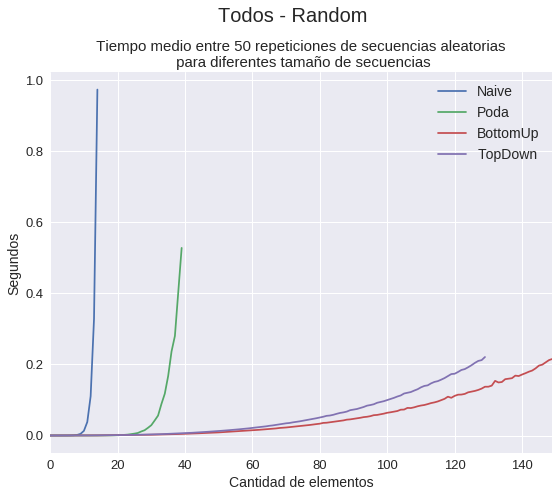
\includegraphics[width=0.75\textwidth]{informe/img/experimentos/todos-random.png} \\
} 

Era esperable que el algoritmo con \textit{poda} sea mucho mas eficiente que el algoritmo \textit{naive}, pero veamos mas de cerca que pasa con los de programación dinámica: \\

% ESTE PODRIA SACARSE PARA AHORRAR LUGAR ... 
% {\centering
%   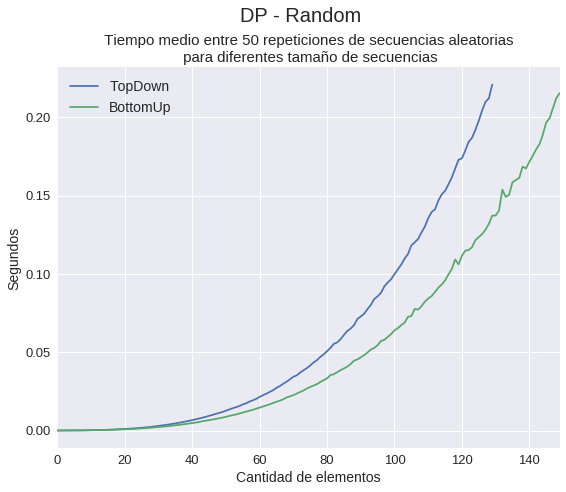
\includegraphics[width=0.75\textwidth]{informe/img/experimentos/dp-random.png} \\
% }

Para instancias de tamaño $\leq 40$ \textit{BottomUp} y \textit{TopDown} se comportan de manera muy similar, pero para tamaños mas grandes las curvas comienzan a separarse. \\

En el análisis teórico, tanto \textit{TopDown} como \textit{BottomUp} tenían la misma complejidad. Lo que podemos deducir de estas mediciones es que \textit{TopDown} tiene una constante oculta mas elevada. Esto es razonable ya que en esta técnica se realizan llamados recursivos y en \textit{BottomUp} no. 

\subsection{Elementos iguales}

En una secuencia donde todos los elementos son iguales, como máximo pueden pintarse un elemento de rojo y otro de azul, pero no más que esto ya que no es posible encontrar secuencias \textit{estrictamente} crecientes o decrecientes. Podríamos considerar esto un mejor caso, ya que en rasgos generales, las técnicas que revisan la validez de la secuencia a medida que la construyen solo podrían ''entrar'' en la rama donde los elementos no se pintan. \\

El algoritmo de \textit{backtracking naive} tiene tiempos tan malos que no permiten ver con claridad las diferencias entre las otras técnicas, por lo que el gráfico está en \textbf{escala logarítmica} en el eje $y$. \\

En el gráfico podemos ver cómo el \textit{backtracking con poda} es el que produce los resultados mas eficientes. Esto es razonable si consideramos la observación del primer párrafo, y si tenemos en cuenta que los algoritmos de \textit{programación dinámica} siempre crean una matriz de tres dimensiones de tamaño $n^3$, sin importar el contenido de la secuencia. \\

% {\centering
%   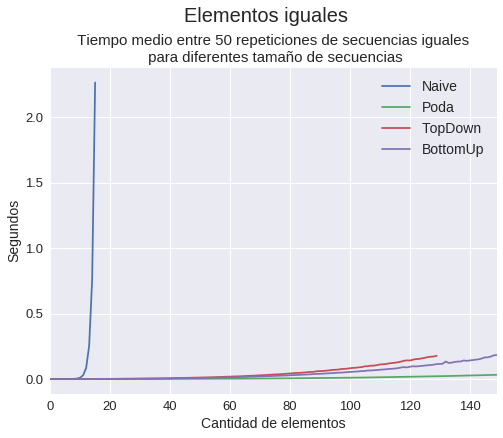
\includegraphics[width=0.75\textwidth]{informe/img/experimentos/todos-iguales.png} \\
% }

{\centering
  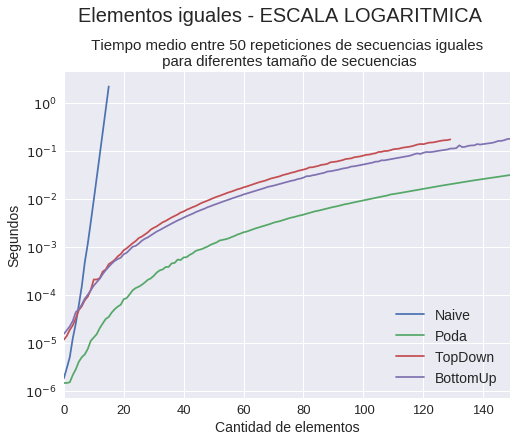
\includegraphics[width=0.75\textwidth]{informe/img/experimentos/todos-iguales-logaritmica.png} \\
}


\end{document}
